\section{寄存器描述}
\regover{
{\hyperref[usb-usb-config]{usb\_config}}&USB configuration
\\
\hline
{\hyperref[usb-usb-lpm-config]{usb\_lpm\_config}}&USB lpm configuration
\\
\hline
{\hyperref[usb-usb-resume-config]{usb\_resume\_config}}&USB resume configuration
\\
\hline
{\hyperref[usb-usb-frame-no]{usb\_frame\_no}}&USB frame number
\\
\hline
{\hyperref[usb-usb-error]{usb\_error}}&USB error
\\
\hline
{\hyperref[usb-usb-int-en]{usb\_int\_en}}&USB interrupt enable
\\
\hline
{\hyperref[usb-usb-int-sts]{usb\_int\_sts}}&USB interrupt status
\\
\hline
{\hyperref[usb-usb-int-mask]{usb\_int\_mask}}&USB interrupt mask
\\
\hline
{\hyperref[usb-usb-int-clear]{usb\_int\_clear}}&USB interrupt clear
\\
\hline
{\hyperref[usb-ep1-config]{ep1\_config}}&EP1 configuration
\\
\hline
{\hyperref[usb-ep2-config]{ep2\_config}}&EP2 configuration
\\
\hline
{\hyperref[usb-ep3-config]{ep3\_config}}&EP3 configuration
\\
\hline
{\hyperref[usb-ep4-config]{ep4\_config}}&EP4 configuration
\\
\hline
{\hyperref[usb-ep5-config]{ep5\_config}}&EP5 configuration
\\
\hline
{\hyperref[usb-ep6-config]{ep6\_config}}&EP6 configuration
\\
\hline
{\hyperref[usb-ep7-config]{ep7\_config}}&EP7 configuration
\\
\hline
{\hyperref[usb-ep0-fifo-config]{ep0\_fifo\_config}}&EP0 fifo configuration
\\
\hline
{\hyperref[usb-ep0-fifo-status]{ep0\_fifo\_status}}&EP0 fifo status
\\
\hline
{\hyperref[usb-ep0-tx-fifo-wdata]{ep0\_tx\_fifo\_wdata}}&EP0 tx fifo write data
\\
\hline
{\hyperref[usb-ep0-rx-fifo-rdata]{ep0\_rx\_fifo\_rdata}}&EP0 rx fifo write data
\\
\hline
{\hyperref[usb-ep1-fifo-config]{ep1\_fifo\_config}}&EP1 fifo configuration
\\
\hline
{\hyperref[usb-ep1-fifo-status]{ep1\_fifo\_status}}&EP1 fifo status
\\
\hline
{\hyperref[usb-ep1-tx-fifo-wdata]{ep1\_tx\_fifo\_wdata}}&EP1 tx fifo write data
\\
\hline
{\hyperref[usb-ep1-rx-fifo-rdata]{ep1\_rx\_fifo\_rdata}}&EP1 rx fifo write data
\\
\hline
{\hyperref[usb-ep2-fifo-config]{ep2\_fifo\_config}}&EP2 fifo configuration
\\
\hline
{\hyperref[usb-ep2-fifo-status]{ep2\_fifo\_status}}&EP2 fifo status
\\
\hline
{\hyperref[usb-ep2-tx-fifo-wdata]{ep2\_tx\_fifo\_wdata}}&EP2 tx fifo write data
\\
\hline
{\hyperref[usb-ep2-rx-fifo-rdata]{ep2\_rx\_fifo\_rdata}}&EP2 rx fifo write data
\\
\hline
{\hyperref[usb-ep3-fifo-config]{ep3\_fifo\_config}}&EP3 fifo configuration
\\
\hline
{\hyperref[usb-ep3-fifo-status]{ep3\_fifo\_status}}&EP3 fifo status
\\
\hline
{\hyperref[usb-ep3-tx-fifo-wdata]{ep3\_tx\_fifo\_wdata}}&EP3 tx fifo write data
\\
\hline
{\hyperref[usb-ep3-rx-fifo-rdata]{ep3\_rx\_fifo\_rdata}}&EP3 rx fifo write data
\\
\hline
{\hyperref[usb-ep4-fifo-config]{ep4\_fifo\_config}}&EP4 fifo configuration
\\
\hline
{\hyperref[usb-ep4-fifo-status]{ep4\_fifo\_status}}&EP4 fifo status
\\
\hline
{\hyperref[usb-ep4-tx-fifo-wdata]{ep4\_tx\_fifo\_wdata}}&EP4 tx fifo write data
\\
\hline
{\hyperref[usb-ep4-rx-fifo-rdata]{ep4\_rx\_fifo\_rdata}}&EP4 rx fifo write data
\\
\hline
{\hyperref[usb-ep5-fifo-config]{ep5\_fifo\_config}}&EP5 fifo configuration
\\
\hline
{\hyperref[usb-ep5-fifo-status]{ep5\_fifo\_status}}&EP5 fifo status
\\
\hline
{\hyperref[usb-ep5-tx-fifo-wdata]{ep5\_tx\_fifo\_wdata}}&EP5 tx fifo write data
\\
\hline
{\hyperref[usb-ep5-rx-fifo-rdata]{ep5\_rx\_fifo\_rdata}}&EP5 rx fifo read data
\\
\hline
{\hyperref[usb-ep6-fifo-config]{ep6\_fifo\_config}}&EP6 fifo configuration
\\
\hline
{\hyperref[usb-ep6-fifo-status]{ep6\_fifo\_status}}&EP6 fifo status
\\
\hline
{\hyperref[usb-ep6-tx-fifo-wdata]{ep6\_tx\_fifo\_wdata}}&EP6 tx fifo write data
\\
\hline
{\hyperref[usb-ep6-rx-fifo-rdata]{ep6\_rx\_fifo\_rdata}}&EP6 rx fifo read data
\\
\hline
{\hyperref[usb-ep7-fifo-config]{ep7\_fifo\_config}}&EP7 fifo configuration
\\
\hline
{\hyperref[usb-ep7-fifo-status]{ep7\_fifo\_status}}&EP7 fifo status
\\
\hline
{\hyperref[usb-ep7-tx-fifo-wdata]{ep7\_tx\_fifo\_wdata}}&EP7 tx fifo write data
\\
\hline
{\hyperref[usb-ep7-rx-fifo-rdata]{ep7\_rx\_fifo\_rdata}}&EP7 rx fifo read data
\\
\hline
{\hyperref[usb-xcvr-if-config]{xcvr\_if\_config}}&
\\
\hline
}

\subsection{usb\_config}
\label{usb-usb-config}
地址:0x4000d800
 \begin{figure}[H]
\includegraphics{usb_usb_config.pdf}
\end{figure}

\regdes{31:29&RSVD& & & \\\hline
28&sts\_usb\_ep0\_sw\_rdy&r&1'b0&EP0 transaction ready status bit. Asserted with sw\_rdy, and de-asserted when ACK is sent/received.\\\hline
27&cr\_usb\_ep0\_sw\_rdy&w1c&1'b0&EP0 transaction ready. When NACK is enabled, asserting this bit will allow one packet to be transferred even if NACK is asserted\\\hline
26&cr\_usb\_ep0\_sw\_nack\_out&r/w&1'b0&EP0 OUT/SETUP transaction nack response (SW control mode) \par Note: Should NOT enable both ep0\_sw\_nack\_out and ep0\_sw\_stall at the same time
\\\hline
25&cr\_usb\_ep0\_sw\_nack\_in&r/w&1'b1&EP0 IN transaction nack response (SW control mode) \par Note: Should NOT enable both ep0\_sw\_nack\_in and ep0\_sw\_stall at the same time
\\\hline
24&cr\_usb\_ep0\_sw\_stall&w1c&1'b0&EP0 stall response (SW control mode) \par Note: Should NOT enable both ep0\_sw\_nack\_in/out and ep0\_sw\_stall at the same time
\\\hline
23:16&cr\_usb\_ep0\_sw\_size&r/w&8'd0&EP0 transfer size (SW control mode)\\\hline
15:9&cr\_usb\_ep0\_sw\_addr&r/w&7'd0&EP0 address (SW control mode)\\\hline
8&cr\_usb\_ep0\_sw\_ctrl&r/w&1'b0&EP0 software control enable \par 1'b1: EP0 IN/OUT transaction is fully contolled by SW \par 1'b0: EP0 IN/OUT transaction is controlled by HW
\\\hline
7:5&RSVD& & & \\\hline
4&cr\_usb\_rom\_dct\_en&r/w&1'b1&Enable signal of ROM-based descriptors (don't care if ep0\_sw\_ctrl is asserted) \par 1'b1: USB descriptors stored in ROM will be used \par 1'b0: SW should prepare the descriptors requested by HOST
\\\hline
3:1&RSVD& & & \\\hline
0&cr\_usb\_en&r/w&1'b0&Enable signal of USB function\\\hline

}
\subsection{usb\_lpm\_config}
\label{usb-usb-lpm-config}
地址:0x4000d804
 \begin{figure}[H]
\includegraphics{usb_usb_lpm_config.pdf}
\end{figure}

\regdes{31&sts\_lpm&r&1'b0&LPM status bit\\\hline
30:20&sts\_lpm\_attr&r&11'h0&LPM attributes received in LPM packet\\\hline
19:4&RSVD& & & \\\hline
3:2&cr\_lpm\_resp&r/w&2'd2&Response when LPM packet is received \par 2'd3: NYET \par 2'd2: STALL \par 2'd1: NACK \par 2'd0: ACK
\\\hline
1&cr\_lpm\_resp\_upd&w1c&1'b0&Response update signal (for async concern) \par Assert this bit when cr\_lpm\_resp is updated
\\\hline
0&cr\_lpm\_en&w1c&1'b0&LPM enable signal\\\hline

}
\subsection{usb\_resume\_config}
\label{usb-usb-resume-config}
地址:0x4000d808
 \begin{figure}[H]
\includegraphics{usb_usb_resume_config.pdf}
\end{figure}

\regdes{31&cr\_res\_force&r/w&1'b0&Force to output K-state\\\hline
30:13&RSVD& & & \\\hline
12&cr\_res\_trig&w1c&1'b0&Resume K-state trigger\\\hline
11&RSVD& & & \\\hline
10:0&cr\_res\_width&r/w&11'd26&Resume K-state width (unit: 2.67us)\\\hline

}
\subsection{usb\_frame\_no}
\label{usb-usb-frame-no}
地址:0x4000d818
 \begin{figure}[H]
\includegraphics{usb_usb_frame_no.pdf}
\end{figure}

\regdes{31:20&RSVD& & & \\\hline
19:16&sts\_ep\_no&r&4'd0&Endpoint number of the current transaction\\\hline
15:12&sts\_pid&r&4'd0&PID value of the current transaction\\\hline
11&RSVD& & & \\\hline
10:0&sts\_frame\_no&r&11'h0&Current frame number\\\hline

}
\subsection{usb\_error}
\label{usb-usb-error}
地址:0x4000d81c
 \begin{figure}[H]
\includegraphics{usb_usb_error.pdf}
\end{figure}

\regdes{31:7&RSVD& & & \\\hline
6&crc16\_err&r&1'b0&Data CRC error occurs, cleared by cr\_usb\_err\_clr\\\hline
5&crc5\_err&r&1'b0&Token CRC error occurs, cleared by cr\_usb\_err\_clr\\\hline
4&pid\_cks\_err&r&1'b0&PID check sum error occurs, cleared by cr\_usb\_err\_clr\\\hline
3&pid\_seq\_err&r&1'b0&PID sequence error occurs, cleared by cr\_usb\_err\_clr\\\hline
2&ivld\_ep\_err&r&1'b0&Invalid endpoint error occurs, cleared by cr\_usb\_err\_clr\\\hline
1&xfer\_to\_err&r&1'b0&Transfer time-out error occurs, cleared by cr\_usb\_err\_clr\\\hline
0&utmi\_rx\_err&r&1'b0&UTMI I/F RX error occurs, cleared by cr\_usb\_err\_clr\\\hline

}
\subsection{usb\_int\_en}
\label{usb-usb-int-en}
地址:0x4000d820
 \begin{figure}[H]
\includegraphics{usb_usb_int_en.pdf}
\end{figure}

\regdes{31&cr\_usb\_err\_en&r/w&1'b1&Interrupt enable of usb\_err\_int\\\hline
30&cr\_sof\_3ms\_en&r/w&1'b0&Interrupt enable of sof\_3ms\_int\\\hline
29&cr\_lpm\_pkt\_en&r/w&1'b0&Interrupt enable of lpm\_pkt\_int\\\hline
28&cr\_lpm\_wkup\_en&r/w&1'b0&Interrupt enable of lpm\_wkup\_int\\\hline
27&cr\_usb\_rend\_en&r/w&1'b0&Interrupt enable of usb\_rend\_int\\\hline
26:24&RSVD& & & \\\hline
23&cr\_ep7\_done\_en&r/w&1'b1&Interrupt enable of ep7\_done\_int\\\hline
22&cr\_ep7\_cmd\_en&r/w&1'b1&Interrupt enable of ep7\_cmd\_int\\\hline
21&cr\_ep6\_done\_en&r/w&1'b1&Interrupt enable of ep6\_done\_int\\\hline
20&cr\_ep6\_cmd\_en&r/w&1'b1&Interrupt enable of ep6\_cmd\_int\\\hline
19&cr\_ep5\_done\_en&r/w&1'b1&Interrupt enable of ep5\_done\_int\\\hline
18&cr\_ep5\_cmd\_en&r/w&1'b1&Interrupt enable of ep5\_cmd\_int\\\hline
17&cr\_ep4\_done\_en&r/w&1'b1&Interrupt enable of ep4\_done\_int\\\hline
16&cr\_ep4\_cmd\_en&r/w&1'b1&Interrupt enable of ep4\_cmd\_int\\\hline
15&cr\_ep3\_done\_en&r/w&1'b1&Interrupt enable of ep3\_done\_int\\\hline
14&cr\_ep3\_cmd\_en&r/w&1'b1&Interrupt enable of ep3\_cmd\_int\\\hline
13&cr\_ep2\_done\_en&r/w&1'b1&Interrupt enable of ep2\_done\_int\\\hline
12&cr\_ep2\_cmd\_en&r/w&1'b1&Interrupt enable of ep2\_cmd\_int\\\hline
11&cr\_ep1\_done\_en&r/w&1'b1&Interrupt enable of ep1\_done\_int\\\hline
10&cr\_ep1\_cmd\_en&r/w&1'b1&Interrupt enable of ep1\_cmd\_int\\\hline
9&cr\_ep0\_out\_done\_en&r/w&1'b1&Interrupt enable of ep0\_out\_done\_int\\\hline
8&cr\_ep0\_out\_cmd\_en&r/w&1'b1&Interrupt enable of ep0\_out\_cmd\_int\\\hline
7&cr\_ep0\_in\_done\_en&r/w&1'b1&Interrupt enable of ep0\_in\_done\_int\\\hline
6&cr\_ep0\_in\_cmd\_en&r/w&1'b1&Interrupt enable of ep0\_in\_cmd\_int\\\hline
5&cr\_ep0\_setup\_done\_en&r/w&1'b1&Interrupt enable of ep0\_setup\_done\_int\\\hline
4&cr\_ep0\_setup\_cmd\_en&r/w&1'b1&Interrupt enable of ep0\_setup\_cmd\_int\\\hline
3&cr\_get\_dct\_cmd\_en&r/w&1'b1&Interrupt enable of get\_dct\_cmd\_int\\\hline
2&cr\_vbus\_tgl\_en&r/w&1'b1&Interrupt enable of vbus\_tgl\_int\\\hline
1&cr\_usb\_reset\_en&r/w&1'b1&Interrupt enable of usb\_reset\_int\\\hline
0&cr\_sof\_en&r/w&1'b1&Interrupt enable of sof\_int\\\hline

}
\subsection{usb\_int\_sts}
\label{usb-usb-int-sts}
地址:0x4000d824
 \begin{figure}[H]
\includegraphics{usb_usb_int_sts.pdf}
\end{figure}

\regdes{31&usb\_err\_int&r&1'b0&USB error occurs, check usb\_error for detailed error type\\\hline
30&sof\_3ms\_int&r&1'b0&SOF is absent for 3 ms\\\hline
29&lpm\_pkt\_int&r&1'b0&LPM packet is received\\\hline
28&lpm\_wkup\_int&r&1'b0&LPM resume (wakeup) signal is received\\\hline
27&usb\_rend\_int&r&1'b0&USB reset de-assert is triggered\\\hline
26:24&RSVD& & & \\\hline
23&ep7\_done\_int&r&1'b0&EP7 IN or OUT command is finished\\\hline
22&ep7\_cmd\_int&r&1'b0&EP7 IN or OUT command is received\\\hline
21&ep6\_done\_int&r&1'b0&EP6 IN or OUT command is finished\\\hline
20&ep6\_cmd\_int&r&1'b0&EP6 IN or OUT command is received\\\hline
19&ep5\_done\_int&r&1'b0&EP5 IN or OUT command is finished\\\hline
18&ep5\_cmd\_int&r&1'b0&EP5 IN or OUT command is received\\\hline
17&ep4\_done\_int&r&1'b0&EP4 IN or OUT command is finished\\\hline
16&ep4\_cmd\_int&r&1'b0&EP4 IN or OUT command is received\\\hline
15&ep3\_done\_int&r&1'b0&EP3 IN or OUT command is finished\\\hline
14&ep3\_cmd\_int&r&1'b0&EP3 IN or OUT command is received\\\hline
13&ep2\_done\_int&r&1'b0&EP2 IN or OUT command is finished\\\hline
12&ep2\_cmd\_int&r&1'b0&EP2 IN or OUT command is received\\\hline
11&ep1\_done\_int&r&1'b0&EP1 IN or OUT command is finished\\\hline
10&ep1\_cmd\_int&r&1'b0&EP1 IN or OUT command is received\\\hline
9&ep0\_out\_done\_int&r&1'b0&EP0 OUT command is finished\\\hline
8&ep0\_out\_cmd\_int&r&1'b0&EP0 OUT command is received\\\hline
7&ep0\_in\_done\_int&r&1'b0&EP0 IN command is finished\\\hline
6&ep0\_in\_cmd\_int&r&1'b0&EP0 IN command is received\\\hline
5&ep0\_setup\_done\_int&r&1'b0&EP0 SETUP command is finished\\\hline
4&ep0\_setup\_cmd\_int&r&1'b0&EP0 SETUP command is received\\\hline
3&get\_dct\_cmd\_int&r&1'b0&GET\_DESCRIPTOR command is received\\\hline
2&vbus\_tgl\_int&r&1'b0&VBUS detection is toggled, check 0x1FC[31] for vbus\_detect status\\\hline
1&usb\_reset\_int&r&1'b0&USB reset is triggered\\\hline
0&sof\_int&r&1'b0&SOF is received\\\hline

}
\subsection{usb\_int\_mask}
\label{usb-usb-int-mask}
地址:0x4000d828
 \begin{figure}[H]
\includegraphics{usb_usb_int_mask.pdf}
\end{figure}

\regdes{31&cr\_usb\_err\_mask&r/w&1'b1&Interrupt mask of usb\_err\_int\\\hline
30&cr\_sof\_3ms\_mask&r/w&1'b1&Interrupt mask of sof\_3ms\_int\\\hline
29&cr\_lpm\_pkt\_mask&r/w&1'b1&Interrupt mask of lpm\_pkt\_int\\\hline
28&cr\_lpm\_wkup\_mask&r/w&1'b1&Interrupt mask of lpm\_wkup\_int\\\hline
27&cr\_usb\_rend\_mask&r/w&1'b1&Interrupt mask of usb\_rend\_int\\\hline
26:24&RSVD& & & \\\hline
23&cr\_ep7\_done\_mask&r/w&1'b1&Interrupt mask of ep7\_done\_int\\\hline
22&cr\_ep7\_cmd\_mask&r/w&1'b1&Interrupt mask of ep7\_cmd\_int\\\hline
21&cr\_ep6\_done\_mask&r/w&1'b1&Interrupt mask of ep6\_done\_int\\\hline
20&cr\_ep6\_cmd\_mask&r/w&1'b1&Interrupt mask of ep6\_cmd\_int\\\hline
19&cr\_ep5\_done\_mask&r/w&1'b1&Interrupt mask of ep5\_done\_int\\\hline
18&cr\_ep5\_cmd\_mask&r/w&1'b1&Interrupt mask of ep5\_cmd\_int\\\hline
17&cr\_ep4\_done\_mask&r/w&1'b1&Interrupt mask of ep4\_done\_int\\\hline
16&cr\_ep4\_cmd\_mask&r/w&1'b1&Interrupt mask of ep4\_cmd\_int\\\hline
15&cr\_ep3\_done\_mask&r/w&1'b1&Interrupt mask of ep3\_done\_int\\\hline
14&cr\_ep3\_cmd\_mask&r/w&1'b1&Interrupt mask of ep3\_cmd\_int\\\hline
13&cr\_ep2\_done\_mask&r/w&1'b1&Interrupt mask of ep2\_done\_int\\\hline
12&cr\_ep2\_cmd\_mask&r/w&1'b1&Interrupt mask of ep2\_cmd\_int\\\hline
11&cr\_ep1\_done\_mask&r/w&1'b1&Interrupt mask of ep1\_done\_int\\\hline
10&cr\_ep1\_cmd\_mask&r/w&1'b1&Interrupt mask of ep1\_cmd\_int\\\hline
9&cr\_ep0\_out\_done\_mask&r/w&1'b1&Interrupt mask of ep0\_out\_done\_int\\\hline
8&cr\_ep0\_out\_cmd\_mask&r/w&1'b1&Interrupt mask of ep0\_out\_cmd\_int\\\hline
7&cr\_ep0\_in\_done\_mask&r/w&1'b1&Interrupt mask of ep0\_in\_done\_int\\\hline
6&cr\_ep0\_in\_cmd\_mask&r/w&1'b1&Interrupt mask of ep0\_in\_cmd\_int\\\hline
5&cr\_ep0\_setup\_done\_mask&r/w&1'b1&Interrupt mask of ep0\_setup\_done\_int\\\hline
4&cr\_ep0\_setup\_cmd\_mask&r/w&1'b1&Interrupt mask of ep0\_setup\_cmd\_int\\\hline
3&cr\_get\_dct\_cmd\_mask&r/w&1'b1&Interrupt mask of get\_dct\_cmd\_int\\\hline
2&cr\_vbus\_tgl\_mask&r/w&1'b1&Interrupt mask of vbus\_tgl\_int\\\hline
1&cr\_usb\_reset\_mask&r/w&1'b1&Interrupt mask of usb\_reset\_int\\\hline
0&cr\_sof\_mask&r/w&1'b1&Interrupt mask of sof\_int\\\hline

}
\subsection{usb\_int\_clear}
\label{usb-usb-int-clear}
地址:0x4000d82c
 \begin{figure}[H]
\includegraphics{usb_usb_int_clear.pdf}
\end{figure}

\regdes{31&cr\_usb\_err\_clr&w1c&1'b0&Interrupt clear of usb\_err\_int\\\hline
30&cr\_sof\_3ms\_clr&w1c&1'b0&Interrupt clear of sof\_3ms\_int\\\hline
29&cr\_lpm\_pkt\_clr&w1c&1'b0&Interrupt clear of lpm\_pkt\_int\\\hline
28&cr\_lpm\_wkup\_clr&w1c&1'b0&Interrupt clear of lpm\_wkup\_int\\\hline
27&cr\_usb\_rend\_clr&w1c&1'b0&Interrupt clear of usb\_rend\_int\\\hline
26:24&RSVD& & & \\\hline
23&cr\_ep7\_done\_clr&w1c&1'b0&Interrupt clear of ep7\_done\_int\\\hline
22&cr\_ep7\_cmd\_clr&w1c&1'b0&Interrupt clear of ep7\_cmd\_int\\\hline
21&cr\_ep6\_done\_clr&w1c&1'b0&Interrupt clear of ep6\_done\_int\\\hline
20&cr\_ep6\_cmd\_clr&w1c&1'b0&Interrupt clear of ep6\_cmd\_int\\\hline
19&cr\_ep5\_done\_clr&w1c&1'b0&Interrupt clear of ep5\_done\_int\\\hline
18&cr\_ep5\_cmd\_clr&w1c&1'b0&Interrupt clear of ep5\_cmd\_int\\\hline
17&cr\_ep4\_done\_clr&w1c&1'b0&Interrupt clear of ep4\_done\_int\\\hline
16&cr\_ep4\_cmd\_clr&w1c&1'b0&Interrupt clear of ep4\_cmd\_int\\\hline
15&cr\_ep3\_done\_clr&w1c&1'b0&Interrupt clear of ep3\_done\_int\\\hline
14&cr\_ep3\_cmd\_clr&w1c&1'b0&Interrupt clear of ep3\_cmd\_int\\\hline
13&cr\_ep2\_done\_clr&w1c&1'b0&Interrupt clear of ep2\_done\_int\\\hline
12&cr\_ep2\_cmd\_clr&w1c&1'b0&Interrupt clear of ep2\_cmd\_int\\\hline
11&cr\_ep1\_done\_clr&w1c&1'b0&Interrupt clear of ep1\_done\_int\\\hline
10&cr\_ep1\_cmd\_clr&w1c&1'b0&Interrupt clear of ep1\_cmd\_int\\\hline
9&cr\_ep0\_out\_done\_clr&w1c&1'b0&Interrupt clear of ep0\_out\_done\_int\\\hline
8&cr\_ep0\_out\_cmd\_clr&w1c&1'b0&Interrupt clear of ep0\_out\_cmd\_int\\\hline
7&cr\_ep0\_in\_done\_clr&w1c&1'b0&Interrupt clear of ep0\_in\_done\_int\\\hline
6&cr\_ep0\_in\_cmd\_clr&w1c&1'b0&Interrupt clear of ep0\_in\_cmd\_int\\\hline
5&cr\_ep0\_setup\_done\_clr&w1c&1'b0&Interrupt clear of ep0\_setup\_done\_int\\\hline
4&cr\_ep0\_setup\_cmd\_clr&w1c&1'b0&Interrupt clear of ep0\_setup\_cmd\_int\\\hline
3&cr\_get\_dct\_cmd\_clr&w1c&1'b0&Interrupt clear of get\_dct\_cmd\_int\\\hline
2&cr\_vbus\_tgl\_clr&w1c&1'b0&Interrupt clear of vbus\_tgl\_int\\\hline
1&cr\_usb\_reset\_clr&w1c&1'b0&Interrupt clear of usb\_reset\_int\\\hline
0&cr\_sof\_clr&w1c&1'b0&Interrupt clear of sof\_int\\\hline

}
\subsection{ep1\_config}
\label{usb-ep1-config}
地址:0x4000d840
 \begin{figure}[H]
\includegraphics{usb_ep1_config.pdf}
\end{figure}

\regdes{31:20&RSVD& & & \\\hline
19&sts\_ep1\_rdy&r&1'b0&Endpoint ready status bit. Asserted with ep\_rdy, and de-asserted when ACK is sent/received.\\\hline
18&cr\_ep1\_rdy&w1c&1'b0&Endpoint ready. When Endpoint NACK is enabled, asserting this bit will allow one packet to be transferred\\\hline
17&cr\_ep1\_nack&r/w&1'b1&Endpoint NACK response enable, should not be enabled with STALL at the same time\\\hline
16&cr\_ep1\_stall&r/w&1'b0&Endpoint STALL response enable, should not be enabled with NACK at the same time\\\hline
15:13&cr\_ep1\_type&r/w&3'b100&Endpoint type \par 3'b101: CTRL \par 3'b010: ISO \par 3'b100: BULK \par 3'b000: INT \par Others: Reserved
\\\hline
12:11&cr\_ep1\_dir&r/w&2'b01&Endpoint direction \par 2'b00: Disabled \par 2'b01: IN \par 2'b10: OUT \par 2'b11: Reserved
\\\hline
10:0&cr\_ep1\_size&r/w&11'd64&Endpoint max packet size\\\hline

}
\subsection{ep2\_config}
\label{usb-ep2-config}
地址:0x4000d844
 \begin{figure}[H]
\includegraphics{usb_ep2_config.pdf}
\end{figure}

\regdes{31:20&RSVD& & & \\\hline
19&sts\_ep2\_rdy&r&1'b0&Endpoint ready status bit. Asserted with ep\_rdy, and de-asserted when ACK is sent/received.\\\hline
18&cr\_ep2\_rdy&w1c&1'b0&Endpoint ready. When Endpoint NACK is enabled, asserting this bit will allow one packet to be transferred\\\hline
17&cr\_ep2\_nack&r/w&1'b1&Endpoint NACK response enable, should not be enabled with STALL at the same time\\\hline
16&cr\_ep2\_stall&r/w&1'b0&Endpoint STALL response enable, should not be enabled with NACK at the same time\\\hline
15:13&cr\_ep2\_type&r/w&3'b100&Endpoint type \par 3'b101: CTRL \par 3'b010: ISO \par 3'b100: BULK \par 3'b000: INT \par Others: Reserved
\\\hline
12:11&cr\_ep2\_dir&r/w&2'b01&Endpoint direction \par 2'b00: Disabled \par 2'b01: IN \par 2'b10: OUT \par 2'b11: Reserved
\\\hline
10:0&cr\_ep2\_size&r/w&11'd64&Endpoint max packet size\\\hline

}
\subsection{ep3\_config}
\label{usb-ep3-config}
地址:0x4000d848
 \begin{figure}[H]
\includegraphics{usb_ep3_config.pdf}
\end{figure}

\regdes{31:20&RSVD& & & \\\hline
19&sts\_ep3\_rdy&r&1'b0&Endpoint ready status bit. Asserted with ep\_rdy, and de-asserted when ACK is sent/received.\\\hline
18&cr\_ep3\_rdy&w1c&1'b0&Endpoint ready. When Endpoint NACK is enabled, asserting this bit will allow one packet to be transferred\\\hline
17&cr\_ep3\_nack&r/w&1'b1&Endpoint NACK response enable, should not be enabled with STALL at the same time\\\hline
16&cr\_ep3\_stall&r/w&1'b0&Endpoint STALL response enable, should not be enabled with NACK at the same time\\\hline
15:13&cr\_ep3\_type&r/w&3'b100&Endpoint type \par 3'b101: CTRL \par 3'b010: ISO \par 3'b100: BULK \par 3'b000: INT \par Others: Reserved
\\\hline
12:11&cr\_ep3\_dir&r/w&2'b01&Endpoint direction \par 2'b00: Disabled \par 2'b01: IN \par 2'b10: OUT \par 2'b11: Reserved
\\\hline
10:0&cr\_ep3\_size&r/w&11'd64&Endpoint max packet size\\\hline

}
\subsection{ep4\_config}
\label{usb-ep4-config}
地址:0x4000d84c
 \begin{figure}[H]
\includegraphics{usb_ep4_config.pdf}
\end{figure}

\regdes{31:20&RSVD& & & \\\hline
19&sts\_ep4\_rdy&r&1'b0&Endpoint ready status bit. Asserted with ep\_rdy, and de-asserted when ACK is sent/received.\\\hline
18&cr\_ep4\_rdy&w1c&1'b0&Endpoint ready. When Endpoint NACK is enabled, asserting this bit will allow one packet to be transferred\\\hline
17&cr\_ep4\_nack&r/w&1'b1&Endpoint NACK response enable, should not be enabled with STALL at the same time\\\hline
16&cr\_ep4\_stall&r/w&1'b0&Endpoint STALL response enable, should not be enabled with NACK at the same time\\\hline
15:13&cr\_ep4\_type&r/w&3'b100&Endpoint type \par 3'b101: CTRL \par 3'b010: ISO \par 3'b100: BULK \par 3'b000: INT \par Others: Reserved
\\\hline
12:11&cr\_ep4\_dir&r/w&2'b01&Endpoint direction \par 2'b00: Disabled \par 2'b01: IN \par 2'b10: OUT \par 2'b11: Reserved
\\\hline
10:0&cr\_ep4\_size&r/w&11'd64&Endpoint max packet size\\\hline

}
\subsection{ep5\_config}
\label{usb-ep5-config}
地址:0x4000d850
 \begin{figure}[H]
\includegraphics{usb_ep5_config.pdf}
\end{figure}

\regdes{31:20&RSVD& & & \\\hline
19&sts\_ep5\_rdy&r&1'b0&Endpoint ready status bit. Asserted with ep\_rdy, and de-asserted when ACK is sent/received.\\\hline
18&cr\_ep5\_rdy&w1c&1'b0&Endpoint ready. When Endpoint NACK is enabled, asserting this bit will allow one packet to be transferred\\\hline
17&cr\_ep5\_nack&r/w&1'b1&Endpoint NACK response enable, should not be enabled with STALL at the same time\\\hline
16&cr\_ep5\_stall&r/w&1'b0&Endpoint STALL response enable, should not be enabled with NACK at the same time\\\hline
15:13&cr\_ep5\_type&r/w&3'b100&Endpoint type \par 3'b101: CTRL \par 3'b010: ISO \par 3'b100: BULK \par 3'b000: INT \par Others: Reserved
\\\hline
12:11&cr\_ep5\_dir&r/w&2'b01&Endpoint direction \par 2'b00: Disabled \par 2'b01: IN \par 2'b10: OUT \par 2'b11: Reserved
\\\hline
10:0&cr\_ep5\_size&r/w&11'd64&Endpoint max packet size\\\hline

}
\subsection{ep6\_config}
\label{usb-ep6-config}
地址:0x4000d854
 \begin{figure}[H]
\includegraphics{usb_ep6_config.pdf}
\end{figure}

\regdes{31:20&RSVD& & & \\\hline
19&sts\_ep6\_rdy&r&1'b0&Endpoint ready status bit. Asserted with ep\_rdy, and de-asserted when ACK is sent/received.\\\hline
18&cr\_ep6\_rdy&w1c&1'b0&Endpoint ready. When Endpoint NACK is enabled, asserting this bit will allow one packet to be transferred\\\hline
17&cr\_ep6\_nack&r/w&1'b1&Endpoint NACK response enable, should not be enabled with STALL at the same time\\\hline
16&cr\_ep6\_stall&r/w&1'b0&Endpoint STALL response enable, should not be enabled with NACK at the same time\\\hline
15:13&cr\_ep6\_type&r/w&3'b100&Endpoint type \par 3'b101: CTRL \par 3'b010: ISO \par 3'b100: BULK \par 3'b000: INT \par Others: Reserved
\\\hline
12:11&cr\_ep6\_dir&r/w&2'b01&Endpoint direction \par 2'b00: Disabled \par 2'b01: IN \par 2'b10: OUT \par 2'b11: Reserved
\\\hline
10:0&cr\_ep6\_size&r/w&11'd64&Endpoint max packet size\\\hline

}
\subsection{ep7\_config}
\label{usb-ep7-config}
地址:0x4000d858
 \begin{figure}[H]
\includegraphics{usb_ep7_config.pdf}
\end{figure}

\regdes{31:20&RSVD& & & \\\hline
19&sts\_ep7\_rdy&r&1'b0&Endpoint ready status bit. Asserted with ep\_rdy, and de-asserted when ACK is sent/received.\\\hline
18&cr\_ep7\_rdy&w1c&1'b0&Endpoint ready. When Endpoint NACK is enabled, asserting this bit will allow one packet to be transferred\\\hline
17&cr\_ep7\_nack&r/w&1'b1&Endpoint NACK response enable, should not be enabled with STALL at the same time\\\hline
16&cr\_ep7\_stall&r/w&1'b0&Endpoint STALL response enable, should not be enabled with NACK at the same time\\\hline
15:13&cr\_ep7\_type&r/w&3'b100&Endpoint type \par 3'b101: CTRL \par 3'b010: ISO \par 3'b100: BULK \par 3'b000: INT \par Others: Reserved
\\\hline
12:11&cr\_ep7\_dir&r/w&2'b01&Endpoint direction \par 2'b00: Disabled \par 2'b01: IN \par 2'b10: OUT \par 2'b11: Reserved
\\\hline
10:0&cr\_ep7\_size&r/w&11'd64&Endpoint max packet size\\\hline

}
\subsection{ep0\_fifo\_config}
\label{usb-ep0-fifo-config}
地址:0x4000d900
 \begin{figure}[H]
\includegraphics{usb_ep0_fifo_config.pdf}
\end{figure}

\regdes{31:8&RSVD& & & \\\hline
7&ep0\_rx\_fifo\_underflow&r&1'b0&Underflow flag of RX FIFO, can be cleared by rx\_fifo\_clr\\\hline
6&ep0\_rx\_fifo\_overflow&r&1'b0&Overflow flag of RX FIFO, can be cleared by rx\_fifo\_clr\\\hline
5&ep0\_tx\_fifo\_underflow&r&1'b0&Underflow flag of TX FIFO, can be cleared by tx\_fifo\_clr\\\hline
4&ep0\_tx\_fifo\_overflow&r&1'b0&Overflow flag of TX FIFO, can be cleared by tx\_fifo\_clr\\\hline
3&ep0\_rx\_fifo\_clr&w1c&1'b0&Clear signal of RX FIFO\\\hline
2&ep0\_tx\_fifo\_clr&w1c&1'b0&Clear signal of TX FIFO\\\hline
1&ep0\_dma\_rx\_en&r/w&1'b0&Enable signal of dma\_rx\_req/ack interface\\\hline
0&ep0\_dma\_tx\_en&r/w&1'b0&Enable signal of dma\_tx\_req/ack interface\\\hline

}
\subsection{ep0\_fifo\_status}
\label{usb-ep0-fifo-status}
地址:0x4000d904
 \begin{figure}[H]
\includegraphics{usb_ep0_fifo_status.pdf}
\end{figure}

\regdes{31&ep0\_rx\_fifo\_full&r&1'b0&RX FIFO full flag\\\hline
30&ep0\_rx\_fifo\_empty&r&1'b1&RX FIFO empty flag\\\hline
29:23&RSVD& & & \\\hline
22:16&ep0\_rx\_fifo\_cnt&r&7'd0&RX FIFO available count\\\hline
15&ep0\_tx\_fifo\_full&r&1'b0&TX FIFO full flag\\\hline
14&ep0\_tx\_fifo\_empty&r&1'b1&TX FIFO empty flag\\\hline
13:7&RSVD& & & \\\hline
6:0&ep0\_tx\_fifo\_cnt&r&7'd64&TX FIFO available count\\\hline

}
\subsection{ep0\_tx\_fifo\_wdata}
\label{usb-ep0-tx-fifo-wdata}
地址:0x4000d908
 \begin{figure}[H]
\includegraphics{usb_ep0_tx_fifo_wdata.pdf}
\end{figure}

\regdes{31:8&RSVD& & & \\\hline
7:0&ep0\_tx\_fifo\_wdata&w&x&\\\hline

}
\subsection{ep0\_rx\_fifo\_rdata}
\label{usb-ep0-rx-fifo-rdata}
地址:0x4000d90c
 \begin{figure}[H]
\includegraphics{usb_ep0_rx_fifo_rdata.pdf}
\end{figure}

\regdes{31:8&RSVD& & & \\\hline
7:0&ep0\_rx\_fifo\_rdata&r&8'h0&\\\hline

}
\subsection{ep1\_fifo\_config}
\label{usb-ep1-fifo-config}
地址:0x4000d910
 \begin{figure}[H]
\includegraphics{usb_ep1_fifo_config.pdf}
\end{figure}

\regdes{31:8&RSVD& & & \\\hline
7&ep1\_rx\_fifo\_underflow&r&1'b0&Underflow flag of RX FIFO, can be cleared by rx\_fifo\_clr\\\hline
6&ep1\_rx\_fifo\_overflow&r&1'b0&Overflow flag of RX FIFO, can be cleared by rx\_fifo\_clr\\\hline
5&ep1\_tx\_fifo\_underflow&r&1'b0&Underflow flag of TX FIFO, can be cleared by tx\_fifo\_clr\\\hline
4&ep1\_tx\_fifo\_overflow&r&1'b0&Overflow flag of TX FIFO, can be cleared by tx\_fifo\_clr\\\hline
3&ep1\_rx\_fifo\_clr&w1c&1'b0&Clear signal of RX FIFO\\\hline
2&ep1\_tx\_fifo\_clr&w1c&1'b0&Clear signal of TX FIFO\\\hline
1&ep1\_dma\_rx\_en&r/w&1'b0&Enable signal of dma\_rx\_req/ack interface\\\hline
0&ep1\_dma\_tx\_en&r/w&1'b0&Enable signal of dma\_tx\_req/ack interface\\\hline

}
\subsection{ep1\_fifo\_status}
\label{usb-ep1-fifo-status}
地址:0x4000d914
 \begin{figure}[H]
\includegraphics{usb_ep1_fifo_status.pdf}
\end{figure}

\regdes{31&ep1\_rx\_fifo\_full&r&1'b0&RX FIFO full flag\\\hline
30&ep1\_rx\_fifo\_empty&r&1'b1&RX FIFO empty flag\\\hline
29:23&RSVD& & & \\\hline
22:16&ep1\_rx\_fifo\_cnt&r&7'd0&RX FIFO available count\\\hline
15&ep1\_tx\_fifo\_full&r&1'b0&TX FIFO full flag\\\hline
14&ep1\_tx\_fifo\_empty&r&1'b1&TX FIFO empty flag\\\hline
13:7&RSVD& & & \\\hline
6:0&ep1\_tx\_fifo\_cnt&r&7'd64&TX FIFO available count\\\hline

}
\subsection{ep1\_tx\_fifo\_wdata}
\label{usb-ep1-tx-fifo-wdata}
地址:0x4000d918
 \begin{figure}[H]
\includegraphics{usb_ep1_tx_fifo_wdata.pdf}
\end{figure}

\regdes{31:8&RSVD& & & \\\hline
7:0&ep1\_tx\_fifo\_wdata&w&x&\\\hline

}
\subsection{ep1\_rx\_fifo\_rdata}
\label{usb-ep1-rx-fifo-rdata}
地址:0x4000d91c
 \begin{figure}[H]
\includegraphics{usb_ep1_rx_fifo_rdata.pdf}
\end{figure}

\regdes{31:8&RSVD& & & \\\hline
7:0&ep1\_rx\_fifo\_rdata&r&8'h0&\\\hline

}
\subsection{ep2\_fifo\_config}
\label{usb-ep2-fifo-config}
地址:0x4000d920
 \begin{figure}[H]
\includegraphics{usb_ep2_fifo_config.pdf}
\end{figure}

\regdes{31:8&RSVD& & & \\\hline
7&ep2\_rx\_fifo\_underflow&r&1'b0&Underflow flag of RX FIFO, can be cleared by rx\_fifo\_clr\\\hline
6&ep2\_rx\_fifo\_overflow&r&1'b0&Overflow flag of RX FIFO, can be cleared by rx\_fifo\_clr\\\hline
5&ep2\_tx\_fifo\_underflow&r&1'b0&Underflow flag of TX FIFO, can be cleared by tx\_fifo\_clr\\\hline
4&ep2\_tx\_fifo\_overflow&r&1'b0&Overflow flag of TX FIFO, can be cleared by tx\_fifo\_clr\\\hline
3&ep2\_rx\_fifo\_clr&w1c&1'b0&Clear signal of RX FIFO\\\hline
2&ep2\_tx\_fifo\_clr&w1c&1'b0&Clear signal of TX FIFO\\\hline
1&ep2\_dma\_rx\_en&r/w&1'b0&Enable signal of dma\_rx\_req/ack interface\\\hline
0&ep2\_dma\_tx\_en&r/w&1'b0&Enable signal of dma\_tx\_req/ack interface\\\hline

}
\subsection{ep2\_fifo\_status}
\label{usb-ep2-fifo-status}
地址:0x4000d924
 \begin{figure}[H]
\includegraphics{usb_ep2_fifo_status.pdf}
\end{figure}

\regdes{31&ep2\_rx\_fifo\_full&r&1'b0&RX FIFO full flag\\\hline
30&ep2\_rx\_fifo\_empty&r&1'b1&RX FIFO empty flag\\\hline
29:23&RSVD& & & \\\hline
22:16&ep2\_rx\_fifo\_cnt&r&7'd0&RX FIFO available count\\\hline
15&ep2\_tx\_fifo\_full&r&1'b0&TX FIFO full flag\\\hline
14&ep2\_tx\_fifo\_empty&r&1'b1&TX FIFO empty flag\\\hline
13:7&RSVD& & & \\\hline
6:0&ep2\_tx\_fifo\_cnt&r&7'd64&TX FIFO available count\\\hline

}
\subsection{ep2\_tx\_fifo\_wdata}
\label{usb-ep2-tx-fifo-wdata}
地址:0x4000d928
 \begin{figure}[H]
\includegraphics{usb_ep2_tx_fifo_wdata.pdf}
\end{figure}

\regdes{31:8&RSVD& & & \\\hline
7:0&ep2\_tx\_fifo\_wdata&w&x&\\\hline

}
\subsection{ep2\_rx\_fifo\_rdata}
\label{usb-ep2-rx-fifo-rdata}
地址:0x4000d92c
 \begin{figure}[H]
\includegraphics{usb_ep2_rx_fifo_rdata.pdf}
\end{figure}

\regdes{31:8&RSVD& & & \\\hline
7:0&ep2\_rx\_fifo\_rdata&r&8'h0&\\\hline

}
\subsection{ep3\_fifo\_config}
\label{usb-ep3-fifo-config}
地址:0x4000d930
 \begin{figure}[H]
\includegraphics{usb_ep3_fifo_config.pdf}
\end{figure}

\regdes{31:8&RSVD& & & \\\hline
7&ep3\_rx\_fifo\_underflow&r&1'b0&Underflow flag of RX FIFO, can be cleared by rx\_fifo\_clr\\\hline
6&ep3\_rx\_fifo\_overflow&r&1'b0&Overflow flag of RX FIFO, can be cleared by rx\_fifo\_clr\\\hline
5&ep3\_tx\_fifo\_underflow&r&1'b0&Underflow flag of TX FIFO, can be cleared by tx\_fifo\_clr\\\hline
4&ep3\_tx\_fifo\_overflow&r&1'b0&Overflow flag of TX FIFO, can be cleared by tx\_fifo\_clr\\\hline
3&ep3\_rx\_fifo\_clr&w1c&1'b0&Clear signal of RX FIFO\\\hline
2&ep3\_tx\_fifo\_clr&w1c&1'b0&Clear signal of TX FIFO\\\hline
1&ep3\_dma\_rx\_en&r/w&1'b0&Enable signal of dma\_rx\_req/ack interface\\\hline
0&ep3\_dma\_tx\_en&r/w&1'b0&Enable signal of dma\_tx\_req/ack interface\\\hline

}
\subsection{ep3\_fifo\_status}
\label{usb-ep3-fifo-status}
地址:0x4000d934
 \begin{figure}[H]
\includegraphics{usb_ep3_fifo_status.pdf}
\end{figure}

\regdes{31&ep3\_rx\_fifo\_full&r&1'b0&RX FIFO full flag\\\hline
30&ep3\_rx\_fifo\_empty&r&1'b1&RX FIFO empty flag\\\hline
29:23&RSVD& & & \\\hline
22:16&ep3\_rx\_fifo\_cnt&r&7'd0&RX FIFO available count\\\hline
15&ep3\_tx\_fifo\_full&r&1'b0&TX FIFO full flag\\\hline
14&ep3\_tx\_fifo\_empty&r&1'b1&TX FIFO empty flag\\\hline
13:7&RSVD& & & \\\hline
6:0&ep3\_tx\_fifo\_cnt&r&7'd64&TX FIFO available count\\\hline

}
\subsection{ep3\_tx\_fifo\_wdata}
\label{usb-ep3-tx-fifo-wdata}
地址:0x4000d938
 \begin{figure}[H]
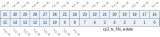
\includegraphics{usb_ep3_tx_fifo_wdata.pdf}
\end{figure}

\regdes{31:8&RSVD& & & \\\hline
7:0&ep3\_tx\_fifo\_wdata&w&x&\\\hline

}
\subsection{ep3\_rx\_fifo\_rdata}
\label{usb-ep3-rx-fifo-rdata}
地址:0x4000d93c
 \begin{figure}[H]
\includegraphics{usb_ep3_rx_fifo_rdata.pdf}
\end{figure}

\regdes{31:8&RSVD& & & \\\hline
7:0&ep3\_rx\_fifo\_rdata&r&8'h0&\\\hline

}
\subsection{ep4\_fifo\_config}
\label{usb-ep4-fifo-config}
地址:0x4000d940
 \begin{figure}[H]
\includegraphics{usb_ep4_fifo_config.pdf}
\end{figure}

\regdes{31:8&RSVD& & & \\\hline
7&ep4\_rx\_fifo\_underflow&r&1'b0&Underflow flag of RX FIFO, can be cleared by rx\_fifo\_clr\\\hline
6&ep4\_rx\_fifo\_overflow&r&1'b0&Overflow flag of RX FIFO, can be cleared by rx\_fifo\_clr\\\hline
5&ep4\_tx\_fifo\_underflow&r&1'b0&Underflow flag of TX FIFO, can be cleared by tx\_fifo\_clr\\\hline
4&ep4\_tx\_fifo\_overflow&r&1'b0&Overflow flag of TX FIFO, can be cleared by tx\_fifo\_clr\\\hline
3&ep4\_rx\_fifo\_clr&w1c&1'b0&Clear signal of RX FIFO\\\hline
2&ep4\_tx\_fifo\_clr&w1c&1'b0&Clear signal of TX FIFO\\\hline
1&ep4\_dma\_rx\_en&r/w&1'b0&Enable signal of dma\_rx\_req/ack interface\\\hline
0&ep4\_dma\_tx\_en&r/w&1'b0&Enable signal of dma\_tx\_req/ack interface\\\hline

}
\subsection{ep4\_fifo\_status}
\label{usb-ep4-fifo-status}
地址:0x4000d944
 \begin{figure}[H]
\includegraphics{usb_ep4_fifo_status.pdf}
\end{figure}

\regdes{31&ep4\_rx\_fifo\_full&r&1'b0&RX FIFO full flag\\\hline
30&ep4\_rx\_fifo\_empty&r&1'b1&RX FIFO empty flag\\\hline
29:23&RSVD& & & \\\hline
22:16&ep4\_rx\_fifo\_cnt&r&7'd0&RX FIFO available count\\\hline
15&ep4\_tx\_fifo\_full&r&1'b0&TX FIFO full flag\\\hline
14&ep4\_tx\_fifo\_empty&r&1'b1&TX FIFO empty flag\\\hline
13:7&RSVD& & & \\\hline
6:0&ep4\_tx\_fifo\_cnt&r&7'd64&TX FIFO available count\\\hline

}
\subsection{ep4\_tx\_fifo\_wdata}
\label{usb-ep4-tx-fifo-wdata}
地址:0x4000d948
 \begin{figure}[H]
\includegraphics{usb_ep4_tx_fifo_wdata.pdf}
\end{figure}

\regdes{31:8&RSVD& & & \\\hline
7:0&ep4\_tx\_fifo\_wdata&w&x&\\\hline

}
\subsection{ep4\_rx\_fifo\_rdata}
\label{usb-ep4-rx-fifo-rdata}
地址:0x4000d94c
 \begin{figure}[H]
\includegraphics{usb_ep4_rx_fifo_rdata.pdf}
\end{figure}

\regdes{31:8&RSVD& & & \\\hline
7:0&ep4\_rx\_fifo\_rdata&r&8'h0&\\\hline

}
\subsection{ep5\_fifo\_config}
\label{usb-ep5-fifo-config}
地址:0x4000d950
 \begin{figure}[H]
\includegraphics{usb_ep5_fifo_config.pdf}
\end{figure}

\regdes{31:8&RSVD& & & \\\hline
7&ep5\_rx\_fifo\_underflow&r&1'b0&Underflow flag of RX FIFO, can be cleared by rx\_fifo\_clr\\\hline
6&ep5\_rx\_fifo\_overflow&r&1'b0&Overflow flag of RX FIFO, can be cleared by rx\_fifo\_clr\\\hline
5&ep5\_tx\_fifo\_underflow&r&1'b0&Underflow flag of TX FIFO, can be cleared by tx\_fifo\_clr\\\hline
4&ep5\_tx\_fifo\_overflow&r&1'b0&Overflow flag of TX FIFO, can be cleared by tx\_fifo\_clr\\\hline
3&ep5\_rx\_fifo\_clr&w1c&1'b0&Clear signal of RX FIFO\\\hline
2&ep5\_tx\_fifo\_clr&w1c&1'b0&Clear signal of TX FIFO\\\hline
1&ep5\_dma\_rx\_en&r/w&1'b0&Enable signal of dma\_rx\_req/ack interface\\\hline
0&ep5\_dma\_tx\_en&r/w&1'b0&Enable signal of dma\_tx\_req/ack interface\\\hline

}
\subsection{ep5\_fifo\_status}
\label{usb-ep5-fifo-status}
地址:0x4000d954
 \begin{figure}[H]
\includegraphics{usb_ep5_fifo_status.pdf}
\end{figure}

\regdes{31&ep5\_rx\_fifo\_full&r&1'b0&RX FIFO full flag\\\hline
30&ep5\_rx\_fifo\_empty&r&1'b1&RX FIFO empty flag\\\hline
29:23&RSVD& & & \\\hline
22:16&ep5\_rx\_fifo\_cnt&r&7'd0&RX FIFO available count\\\hline
15&ep5\_tx\_fifo\_full&r&1'b0&TX FIFO full flag\\\hline
14&ep5\_tx\_fifo\_empty&r&1'b1&TX FIFO empty flag\\\hline
13:7&RSVD& & & \\\hline
6:0&ep5\_tx\_fifo\_cnt&r&7'd64&TX FIFO available count\\\hline

}
\subsection{ep5\_tx\_fifo\_wdata}
\label{usb-ep5-tx-fifo-wdata}
地址:0x4000d958
 \begin{figure}[H]
\includegraphics{usb_ep5_tx_fifo_wdata.pdf}
\end{figure}

\regdes{31:8&RSVD& & & \\\hline
7:0&ep5\_tx\_fifo\_wdata&w&x&\\\hline

}
\subsection{ep5\_rx\_fifo\_rdata}
\label{usb-ep5-rx-fifo-rdata}
地址:0x4000d95c
 \begin{figure}[H]
\includegraphics{usb_ep5_rx_fifo_rdata.pdf}
\end{figure}

\regdes{31:8&RSVD& & & \\\hline
7:0&ep5\_rx\_fifo\_rdata&r&8'h0&\\\hline

}
\subsection{ep6\_fifo\_config}
\label{usb-ep6-fifo-config}
地址:0x4000d960
 \begin{figure}[H]
\includegraphics{usb_ep6_fifo_config.pdf}
\end{figure}

\regdes{31:8&RSVD& & & \\\hline
7&ep6\_rx\_fifo\_underflow&r&1'b0&Underflow flag of RX FIFO, can be cleared by rx\_fifo\_clr\\\hline
6&ep6\_rx\_fifo\_overflow&r&1'b0&Overflow flag of RX FIFO, can be cleared by rx\_fifo\_clr\\\hline
5&ep6\_tx\_fifo\_underflow&r&1'b0&Underflow flag of TX FIFO, can be cleared by tx\_fifo\_clr\\\hline
4&ep6\_tx\_fifo\_overflow&r&1'b0&Overflow flag of TX FIFO, can be cleared by tx\_fifo\_clr\\\hline
3&ep6\_rx\_fifo\_clr&w1c&1'b0&Clear signal of RX FIFO\\\hline
2&ep6\_tx\_fifo\_clr&w1c&1'b0&Clear signal of TX FIFO\\\hline
1&ep6\_dma\_rx\_en&r/w&1'b0&Enable signal of dma\_rx\_req/ack interface\\\hline
0&ep6\_dma\_tx\_en&r/w&1'b0&Enable signal of dma\_tx\_req/ack interface\\\hline

}
\subsection{ep6\_fifo\_status}
\label{usb-ep6-fifo-status}
地址:0x4000d964
 \begin{figure}[H]
\includegraphics{usb_ep6_fifo_status.pdf}
\end{figure}

\regdes{31&ep6\_rx\_fifo\_full&r&1'b0&RX FIFO full flag\\\hline
30&ep6\_rx\_fifo\_empty&r&1'b1&RX FIFO empty flag\\\hline
29:23&RSVD& & & \\\hline
22:16&ep6\_rx\_fifo\_cnt&r&7'd0&RX FIFO available count\\\hline
15&ep6\_tx\_fifo\_full&r&1'b0&TX FIFO full flag\\\hline
14&ep6\_tx\_fifo\_empty&r&1'b1&TX FIFO empty flag\\\hline
13:7&RSVD& & & \\\hline
6:0&ep6\_tx\_fifo\_cnt&r&7'd64&TX FIFO available count\\\hline

}
\subsection{ep6\_tx\_fifo\_wdata}
\label{usb-ep6-tx-fifo-wdata}
地址:0x4000d968
 \begin{figure}[H]
\includegraphics{usb_ep6_tx_fifo_wdata.pdf}
\end{figure}

\regdes{31:8&RSVD& & & \\\hline
7:0&ep6\_tx\_fifo\_wdata&w&x&\\\hline

}
\subsection{ep6\_rx\_fifo\_rdata}
\label{usb-ep6-rx-fifo-rdata}
地址:0x4000d96c
 \begin{figure}[H]
\includegraphics{usb_ep6_rx_fifo_rdata.pdf}
\end{figure}

\regdes{31:8&RSVD& & & \\\hline
7:0&ep6\_rx\_fifo\_rdata&r&8'h0&\\\hline

}
\subsection{ep7\_fifo\_config}
\label{usb-ep7-fifo-config}
地址:0x4000d970
 \begin{figure}[H]
\includegraphics{usb_ep7_fifo_config.pdf}
\end{figure}

\regdes{31:8&RSVD& & & \\\hline
7&ep7\_rx\_fifo\_underflow&r&1'b0&Underflow flag of RX FIFO, can be cleared by rx\_fifo\_clr\\\hline
6&ep7\_rx\_fifo\_overflow&r&1'b0&Overflow flag of RX FIFO, can be cleared by rx\_fifo\_clr\\\hline
5&ep7\_tx\_fifo\_underflow&r&1'b0&Underflow flag of TX FIFO, can be cleared by tx\_fifo\_clr\\\hline
4&ep7\_tx\_fifo\_overflow&r&1'b0&Overflow flag of TX FIFO, can be cleared by tx\_fifo\_clr\\\hline
3&ep7\_rx\_fifo\_clr&w1c&1'b0&Clear signal of RX FIFO\\\hline
2&ep7\_tx\_fifo\_clr&w1c&1'b0&Clear signal of TX FIFO\\\hline
1&ep7\_dma\_rx\_en&r/w&1'b0&Enable signal of dma\_rx\_req/ack interface\\\hline
0&ep7\_dma\_tx\_en&r/w&1'b0&Enable signal of dma\_tx\_req/ack interface\\\hline

}
\subsection{ep7\_fifo\_status}
\label{usb-ep7-fifo-status}
地址:0x4000d974
 \begin{figure}[H]
\includegraphics{usb_ep7_fifo_status.pdf}
\end{figure}

\regdes{31&ep7\_rx\_fifo\_full&r&1'b0&RX FIFO full flag\\\hline
30&ep7\_rx\_fifo\_empty&r&1'b1&RX FIFO empty flag\\\hline
29:23&RSVD& & & \\\hline
22:16&ep7\_rx\_fifo\_cnt&r&7'd0&RX FIFO available count\\\hline
15&ep7\_tx\_fifo\_full&r&1'b0&TX FIFO full flag\\\hline
14&ep7\_tx\_fifo\_empty&r&1'b1&TX FIFO empty flag\\\hline
13:7&RSVD& & & \\\hline
6:0&ep7\_tx\_fifo\_cnt&r&7'd64&TX FIFO available count\\\hline

}
\subsection{ep7\_tx\_fifo\_wdata}
\label{usb-ep7-tx-fifo-wdata}
地址:0x4000d978
 \begin{figure}[H]
\includegraphics{usb_ep7_tx_fifo_wdata.pdf}
\end{figure}

\regdes{31:8&RSVD& & & \\\hline
7:0&ep7\_tx\_fifo\_wdata&w&x&\\\hline

}
\subsection{ep7\_rx\_fifo\_rdata}
\label{usb-ep7-rx-fifo-rdata}
地址:0x4000d97c
 \begin{figure}[H]
\includegraphics{usb_ep7_rx_fifo_rdata.pdf}
\end{figure}

\regdes{31:8&RSVD& & & \\\hline
7:0&ep7\_rx\_fifo\_rdata&r&8'h0&\\\hline

}
\subsection{xcvr\_if\_config}
\label{usb-xcvr-if-config}
地址:0x4000d9fc
 \begin{figure}[H]
\includegraphics{usb_xcvr_if_config.pdf}
\end{figure}

\regdes{31&sts\_vbus\_det&r&1'b0&Transceiver VBUS detection status\\\hline
30:12&RSVD& & & \\\hline
11&cr\_xcvr\_om\_rx\_dn&r/w&1'b0&Transceiver RX signals output mode CR value\\\hline
10&cr\_xcvr\_om\_rx\_dp&r/w&1'b1&Transceiver RX signals output mode CR value\\\hline
9&cr\_xcvr\_om\_rx\_d&r/w&1'b1&Transceiver RX signals output mode CR value\\\hline
8&cr\_xcvr\_om\_rx\_sel&r/w&1'b0&Select signal of transceiver RX signals in output mode (tx\_oe\# = 0) \par 1'b0: rx\_d/dp/dn is directly from transceiver \par 1'b1: rx\_d/dp/dn is controlled by CR (cr\_xcvr\_om\_rx\_d/dp/dn)
\\\hline
7&cr\_xcvr\_force\_rx\_dn&r/w&1'b0&Transceiver RX signals force mode value\\\hline
6&cr\_xcvr\_force\_rx\_dp&r/w&1'b1&Transceiver RX signals force mode value\\\hline
5&cr\_xcvr\_force\_rx\_d&r/w&1'b1&Transceiver RX signals force mode value\\\hline
4&cr\_xcvr\_force\_rx\_en&r/w&1'b0&Enable signal of transceiver RX signals force mode \par 1'b0: rx\_d/dp/dn is from Transceiver \par 1'b1: tx\_d/dp/dn is controlled by CR (cr\_xcvr\_force\_rx\_d/dp/dn)
\\\hline
3&cr\_xcvr\_force\_tx\_dn&r/w&1'b0&Transceiver TX signals force mode value\\\hline
2&cr\_xcvr\_force\_tx\_dp&r/w&1'b1&Transceiver TX signals force mode value\\\hline
1&cr\_xcvr\_force\_tx\_oe&r/w&1'b0&Transceiver TX signals force mode value\\\hline
0&cr\_xcvr\_force\_tx\_en&r/w&1'b0&Enable signal of transceiver TX signals force mode \par 1'b0: tx\_oe/dp/dn is controlled by HW \par 1'b1: tx\_oe/dp/dn is controlled by CR (cr\_xcvr\_force\_tx\_oe/dp/dn)
\\\hline

}
